\documentclass[aspectratio=169]{beamer}

\usetheme{Madrid}
\usecolortheme{default}

\usepackage[utf8]{inputenc}
\usepackage[T1]{fontenc}
\IfFileExists{spanish.ldf}{%
  \usepackage[spanish,es-noquoting]{babel}%
}{%
  \usepackage[english]{babel}%
}
\usepackage{graphicx}
\usepackage{booktabs}
\usepackage{siunitx}
\usepackage{amsmath}
\usepackage{xcolor}
\usepackage{hyperref}

\sisetup{detect-all}

\title[NA64-mini en Meiga]{Implementación y validación del hodoscopio NA64-mini en Meiga}
\author{René Ríos / Proyecto de Muografía}
\institute{Universidad de La Serena}
\date{\today}

\newcommand{\code}[1]{\texttt{\small #1}}
\newcommand{\ok}{\textcolor{green!45!black}{PASS}}

\begin{document}

\begin{frame}
  \titlepage
\end{frame}

\begin{frame}{Motivación}
  \begin{itemize}
    \item Implementar el hodoscopio NA64-mini dentro de Meiga.
    \item Usar Geant4/Meiga para validar geometría, scoring y coincidencias.
    \item Preparar una base controlada para reconstrucción angular y matriz \(F\).
    \item Evitar la interpretación previa de 8 barras por plano o 32 barras totales.
  \end{itemize}
\end{frame}

\begin{frame}{Objetivo de esta iteración}
  \begin{columns}[T]
    \begin{column}{0.52\textwidth}
      \begin{itemize}
        \item Implementación mínima pero validada.
        \item Geometría activa completa.
        \item Scoring por barra.
        \item Coincidencias X-Y por módulo.
        \item Coincidencia LOWER-UPPER.
      \end{itemize}
    \end{column}
    \begin{column}{0.42\textwidth}
      \begin{block}{Fuera de alcance}
        Sin óptica completa, transporte de fotones, respuesta realista de SiPM,
        pulsos electrónicos ni reconstrucción sub-píxel.
      \end{block}
    \end{column}
  \end{columns}
\end{frame}

\begin{frame}{Geometría global}
  \begin{columns}[T]
    \begin{column}{0.42\textwidth}
      \begin{itemize}
        \item LOWER: \(z = \SI{0.00}{mm}\) a \(\SI{12.00}{mm}\).
        \item UPPER: \(z = \SI{98.40}{mm}\) a \(\SI{110.40}{mm}\).
        \item Separación entre centros: \(\SI{98.40}{mm}\).
        \item Separación libre: \(\SI{86.40}{mm}\).
        \item Espesor por módulo: \(\SI{12.00}{mm}\).
      \end{itemize}
    \end{column}
    \begin{column}{0.56\textwidth}
      \centering
      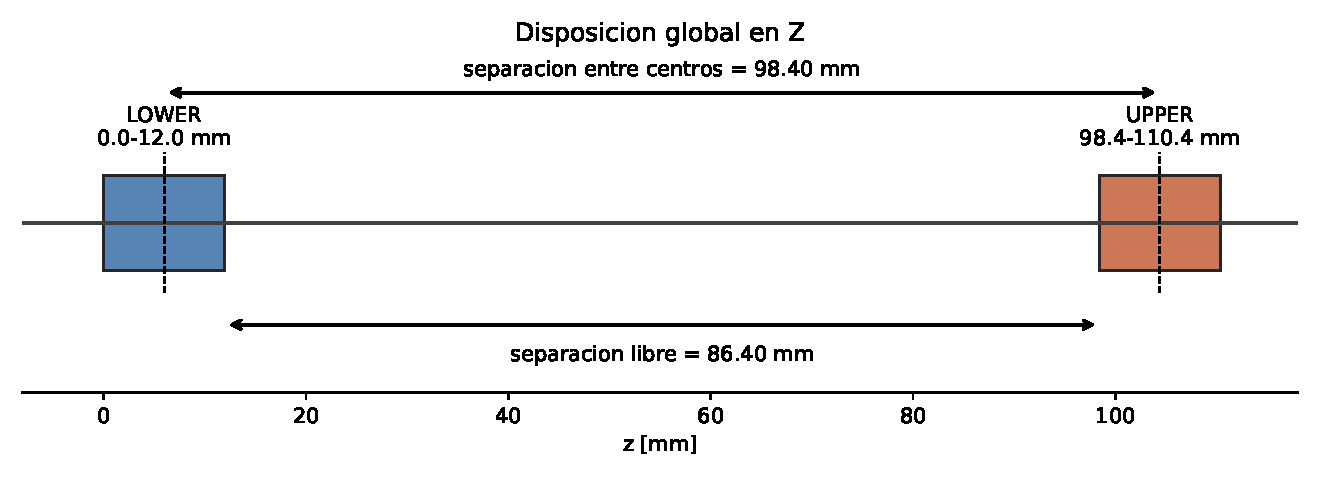
\includegraphics[width=\textwidth]{figures/hodoscope_z_layout.pdf}
    \end{column}
  \end{columns}
\end{frame}

\begin{frame}{Estructura de cada módulo}
  \begin{columns}[T]
    \begin{column}{0.40\textwidth}
      \begin{itemize}
        \item 2 ejes: X e Y.
        \item 16 canales por eje.
        \item 32 barras por módulo.
        \item 64 barras activas totales.
        \item 2 subplanos por eje.
        \item 8 barras por subplano.
        \item Offset lateral: \(\SI{2}{mm}\).
        \item Barras: \(\SI{75 x 3 x 1}{mm}\).
      \end{itemize}
    \end{column}
    \begin{column}{0.58\textwidth}
      \centering
      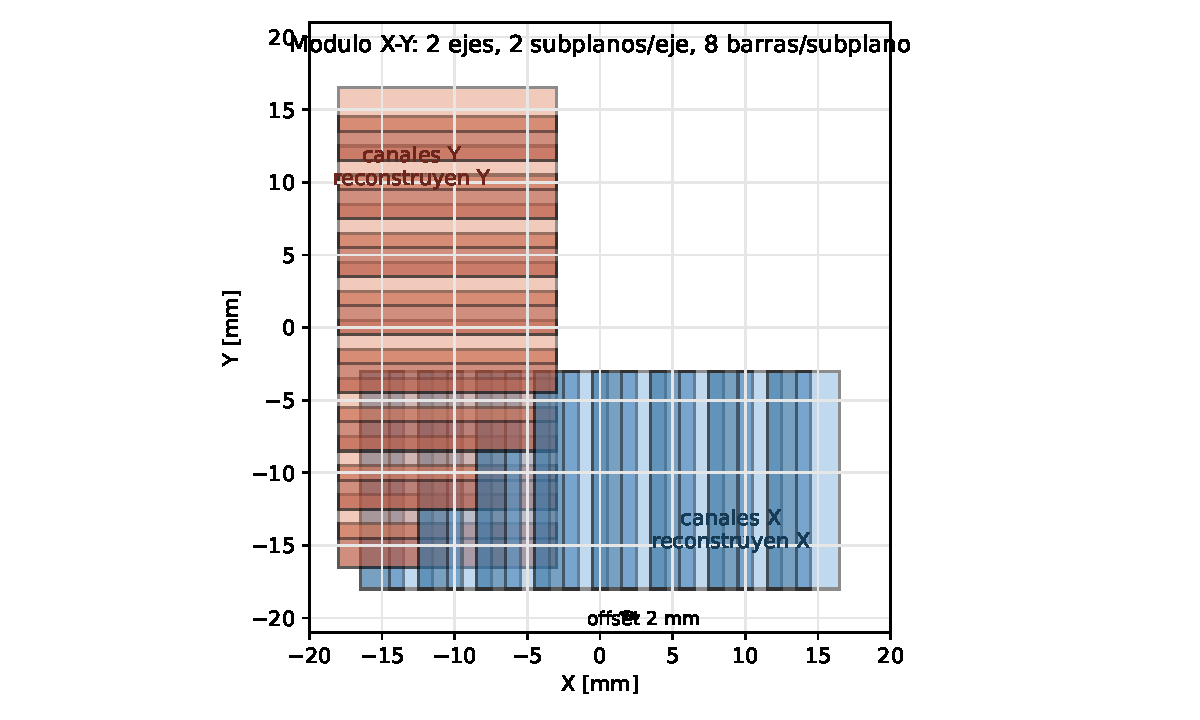
\includegraphics[height=0.72\textheight]{figures/module_xy_structure.pdf}
    \end{column}
  \end{columns}
\end{frame}

\begin{frame}{Convención de canales y píxeles}
  \begin{columns}[T]
    \begin{column}{0.45\textwidth}
      \begin{itemize}
        \item Cada módulo tiene 16 posiciones resolubles en X.
        \item Cada módulo tiene 16 posiciones resolubles en Y.
        \item Matriz discreta por módulo:
          \[
            16 \times 16 = 256 \;\text{píxeles}.
          \]
        \item Identificador:
          \[
            pixel\_id = x + 16\,y.
          \]
        \item El overlap no crea píxeles nuevos; refina posición sub-píxel.
      \end{itemize}
    \end{column}
    \begin{column}{0.52\textwidth}
      \centering
      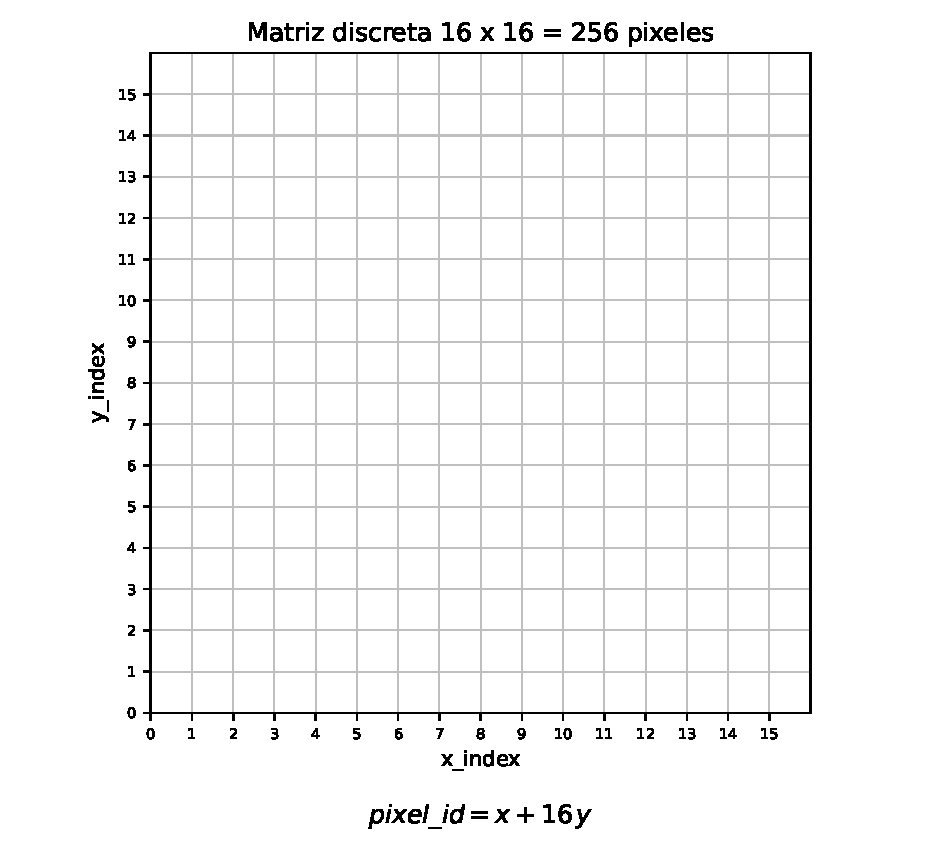
\includegraphics[height=0.70\textheight]{figures/pixel_matrix_16x16.pdf}
    \end{column}
  \end{columns}
\end{frame}

\begin{frame}{Materiales y reflectores}
  \begin{columns}[T]
    \begin{column}{0.52\textwidth}
      \begin{itemize}
        \item Material activo: BC-408 o poliestireno centellador equivalente.
        \item Light yield metadata: \(12800\) photons/MeV.
        \item Attenuation length metadata: \(\SI{2100}{mm}\).
        \item MPPC metadata: Hamamatsu S12572-100P.
      \end{itemize}
    \end{column}
    \begin{column}{0.42\textwidth}
      \begin{block}{Configuración por módulo}
        \begin{tabular}{ll}
          \toprule
          Módulo & Reflector \\
          \midrule
          LOWER & VikuitiESR \\
          UPPER & TiO2Paint \\
          \bottomrule
        \end{tabular}
      \end{block}
      \vspace{0.4em}
      Modo de material muerto actual: \code{active\_only}.
    \end{column}
  \end{columns}
\end{frame}

\begin{frame}{Cambios principales en Meiga}
  \small
  \begin{tabular}{p{0.30\textwidth}p{0.62\textwidth}}
    \toprule
    Archivo & Cambio principal \\
    \midrule
    \code{Hodoscope.cc} & Modo específico \code{NA64Mini}, geometría de dos módulos y 64 barras. \\
    \code{DetectorSimData.h} & Acumuladores por barra y primer tiempo de hit. \\
    \code{DataWriter.cc} & JSON con hits activos, canales, píxeles y coincidencias. \\
    \code{DetectorList.xml} & Configuración del hodoscopio NA64-mini. \\
    \code{analyze\_hodoscope\_output.py} & Diagnóstico de ocupancias, multiplicidades y sanity checks. \\
    \bottomrule
  \end{tabular}
  \vspace{0.8em}

  El modelo se añadió como modo específico de \code{eHodoscope}, preservando la ruta legada.
\end{frame}

\begin{frame}{Validación de geometría}
  \begin{columns}[T]
    \begin{column}{0.52\textwidth}
      \begin{tabular}{lc}
        \toprule
        Check & Resultado \\
        \midrule
        CheckOverlaps & \ok \\
        Total active bars \(=64\) & \ok \\
        LOWER pixels \(=256\) & \ok \\
        UPPER pixels \(=256\) & \ok \\
        UPPER \(\neq\) VikuitiESR & \ok \\
        UPPER \(=\) TiO2Paint & \ok \\
        Rango en \(z\) & \ok \\
        \bottomrule
      \end{tabular}
    \end{column}
    \begin{column}{0.42\textwidth}
      \begin{block}{Resultado}
        La geometría activa compila y corre con \code{CheckOverlaps=true}.
        El log no reportó solapamientos graves.
      \end{block}
    \end{column}
  \end{columns}
\end{frame}

\begin{frame}{Resultados de 1000 eventos}
  \begin{columns}[T]
    \begin{column}{0.44\textwidth}
      \small
      \begin{tabular}{lr}
        \toprule
        Observable & Eventos \\
        \midrule
        LOWER\_X hits & 771 \\
        LOWER\_Y hits & 785 \\
        UPPER\_X hits & 770 \\
        UPPER\_Y hits & 785 \\
        LOWER\_XY & 569 \\
        UPPER\_XY & 568 \\
        FULL & 567 \\
        \bottomrule
      \end{tabular}
    \end{column}
    \begin{column}{0.54\textwidth}
      \centering
      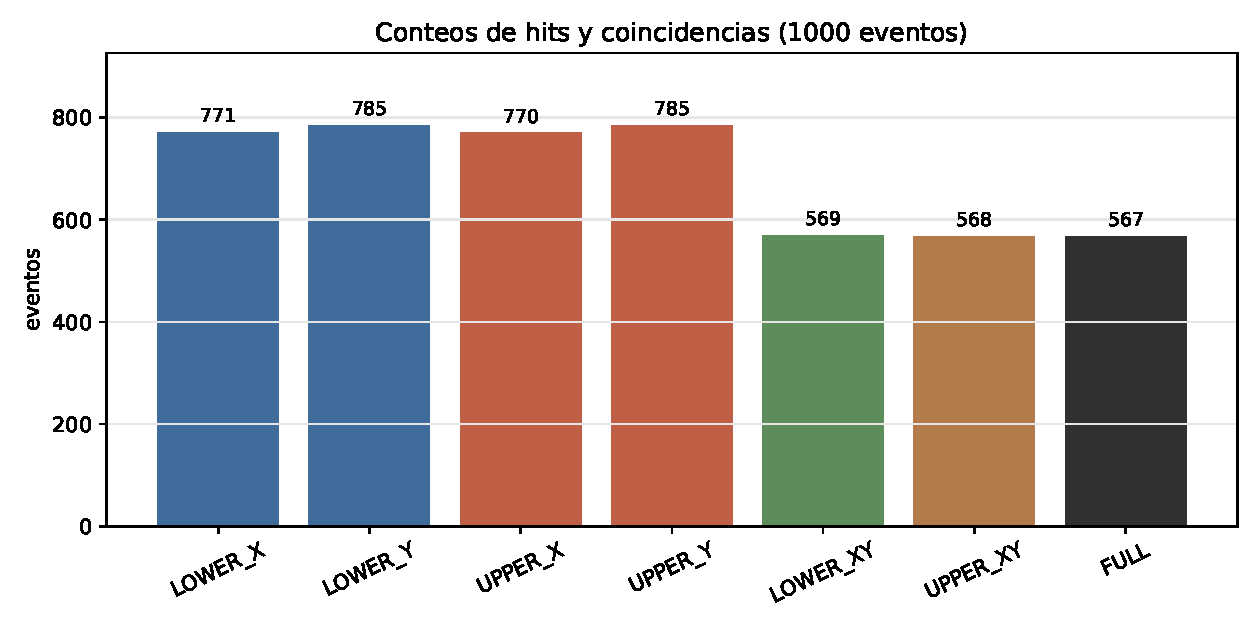
\includegraphics[width=\textwidth]{figures/coincidence_counts.pdf}
    \end{column}
  \end{columns}
\end{frame}

\begin{frame}{Multiplicidad por eje}
  \centering
  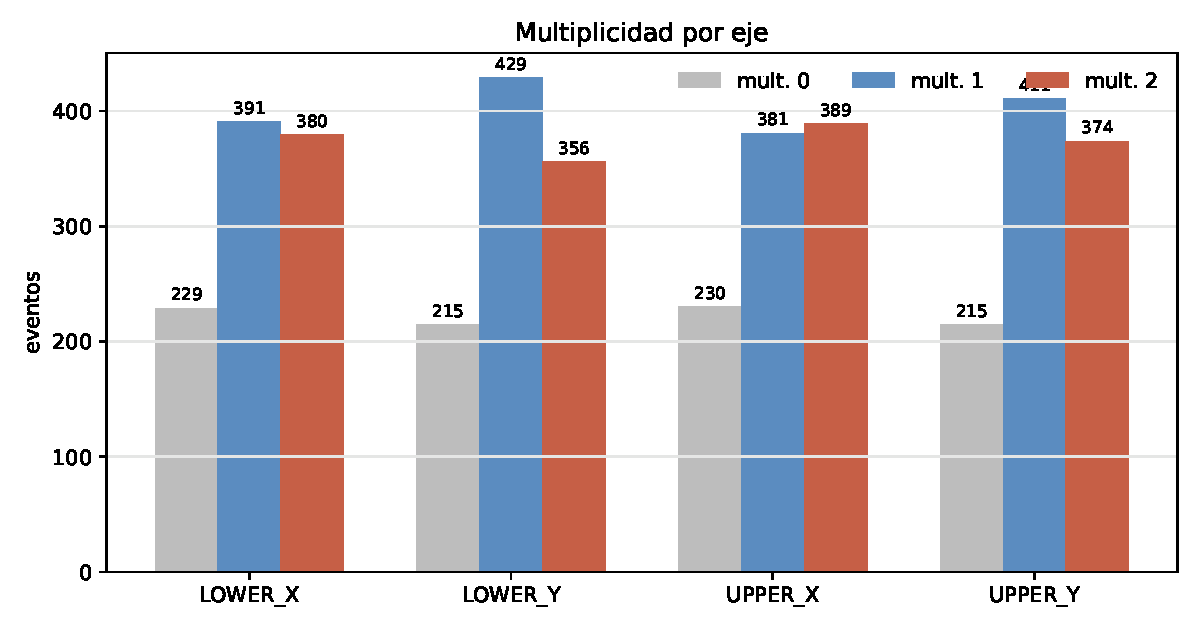
\includegraphics[width=0.88\textwidth]{figures/multiplicity_by_axis.pdf}

  \vspace{0.5em}
  \small
  La multiplicidad 2 aparece de forma natural en zonas de overlap y por la
  presencia de subplanos desplazados.
\end{frame}

\begin{frame}{Ocupancia por barra}
  \centering
  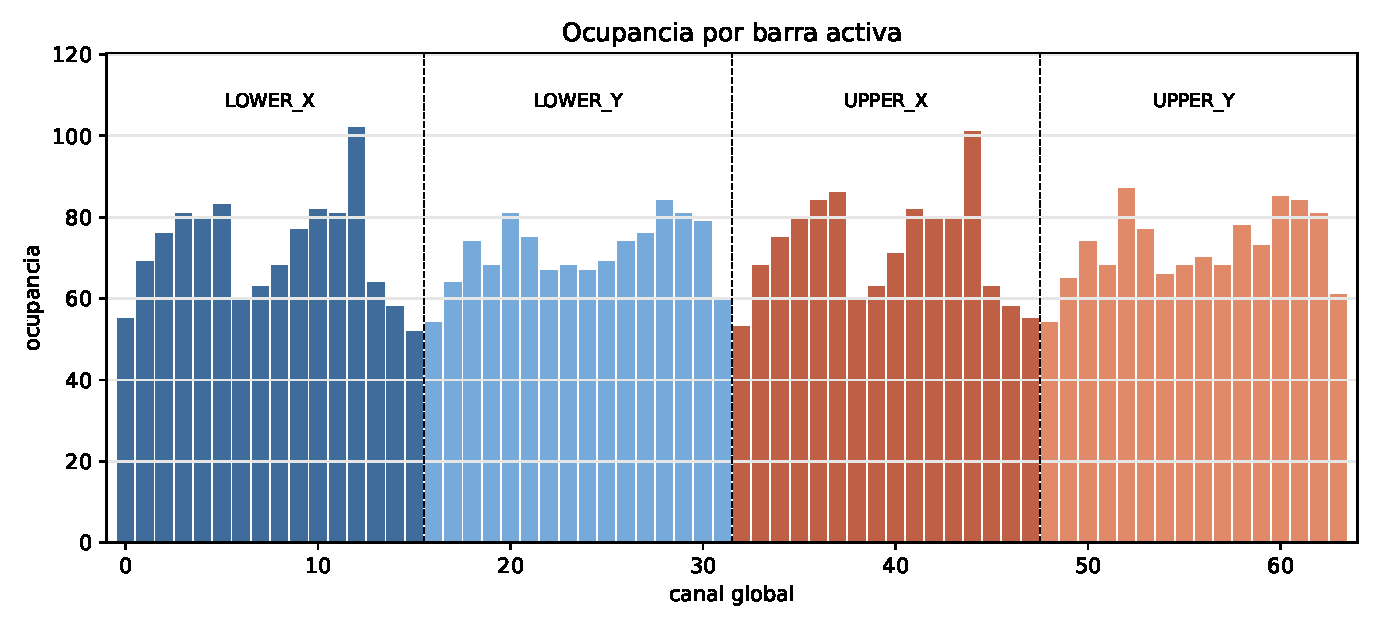
\includegraphics[width=0.92\textwidth]{figures/bar_occupancy.pdf}

  \vspace{0.5em}
  \small
  La numeración global separa visualmente LOWER\_X, LOWER\_Y, UPPER\_X y UPPER\_Y.
\end{frame}

\begin{frame}{Ocupancia de píxeles}
  \begin{columns}[T]
    \begin{column}{0.49\textwidth}
      \centering
      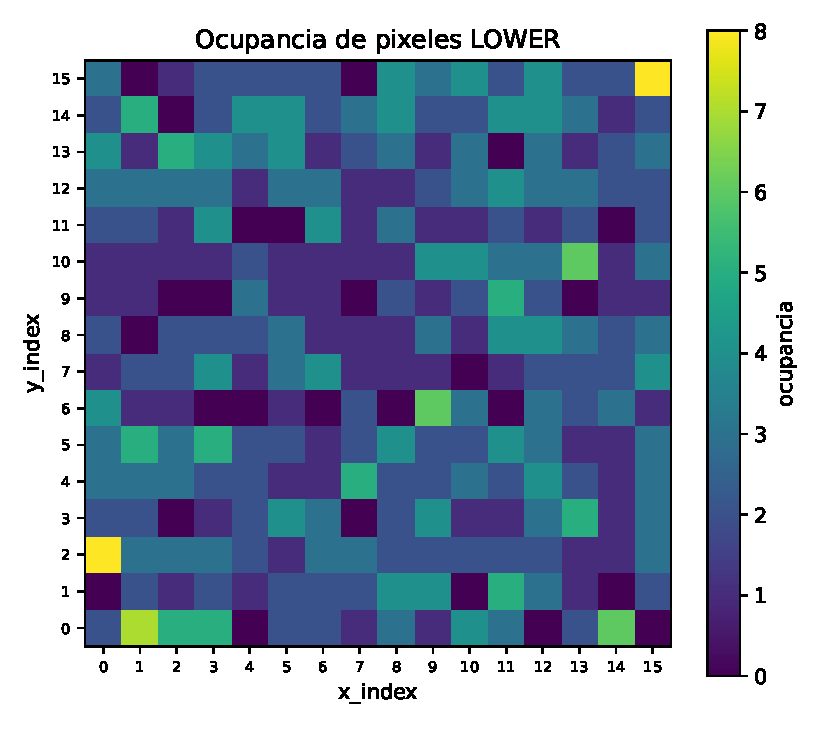
\includegraphics[width=\textwidth]{figures/pixel_occupancy_lower.pdf}

      \small LOWER
    \end{column}
    \begin{column}{0.49\textwidth}
      \centering
      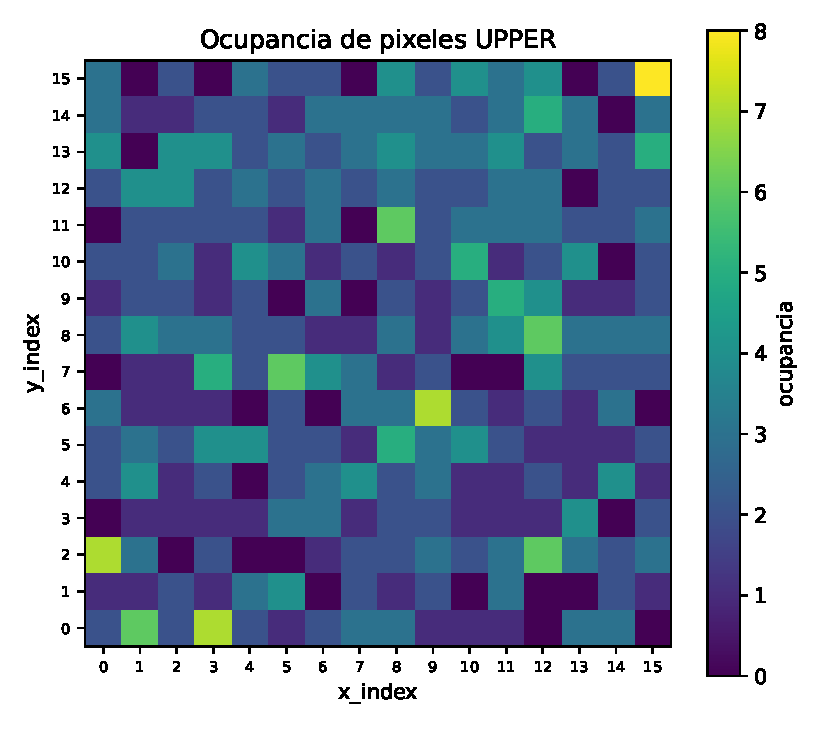
\includegraphics[width=\textwidth]{figures/pixel_occupancy_upper.pdf}

      \small UPPER
    \end{column}
  \end{columns}
\end{frame}

\IfFileExists{figures/meiga_geometry_view.png}{
\begin{frame}{Visualización de geometría en Meiga/Geant4}
  \centering
  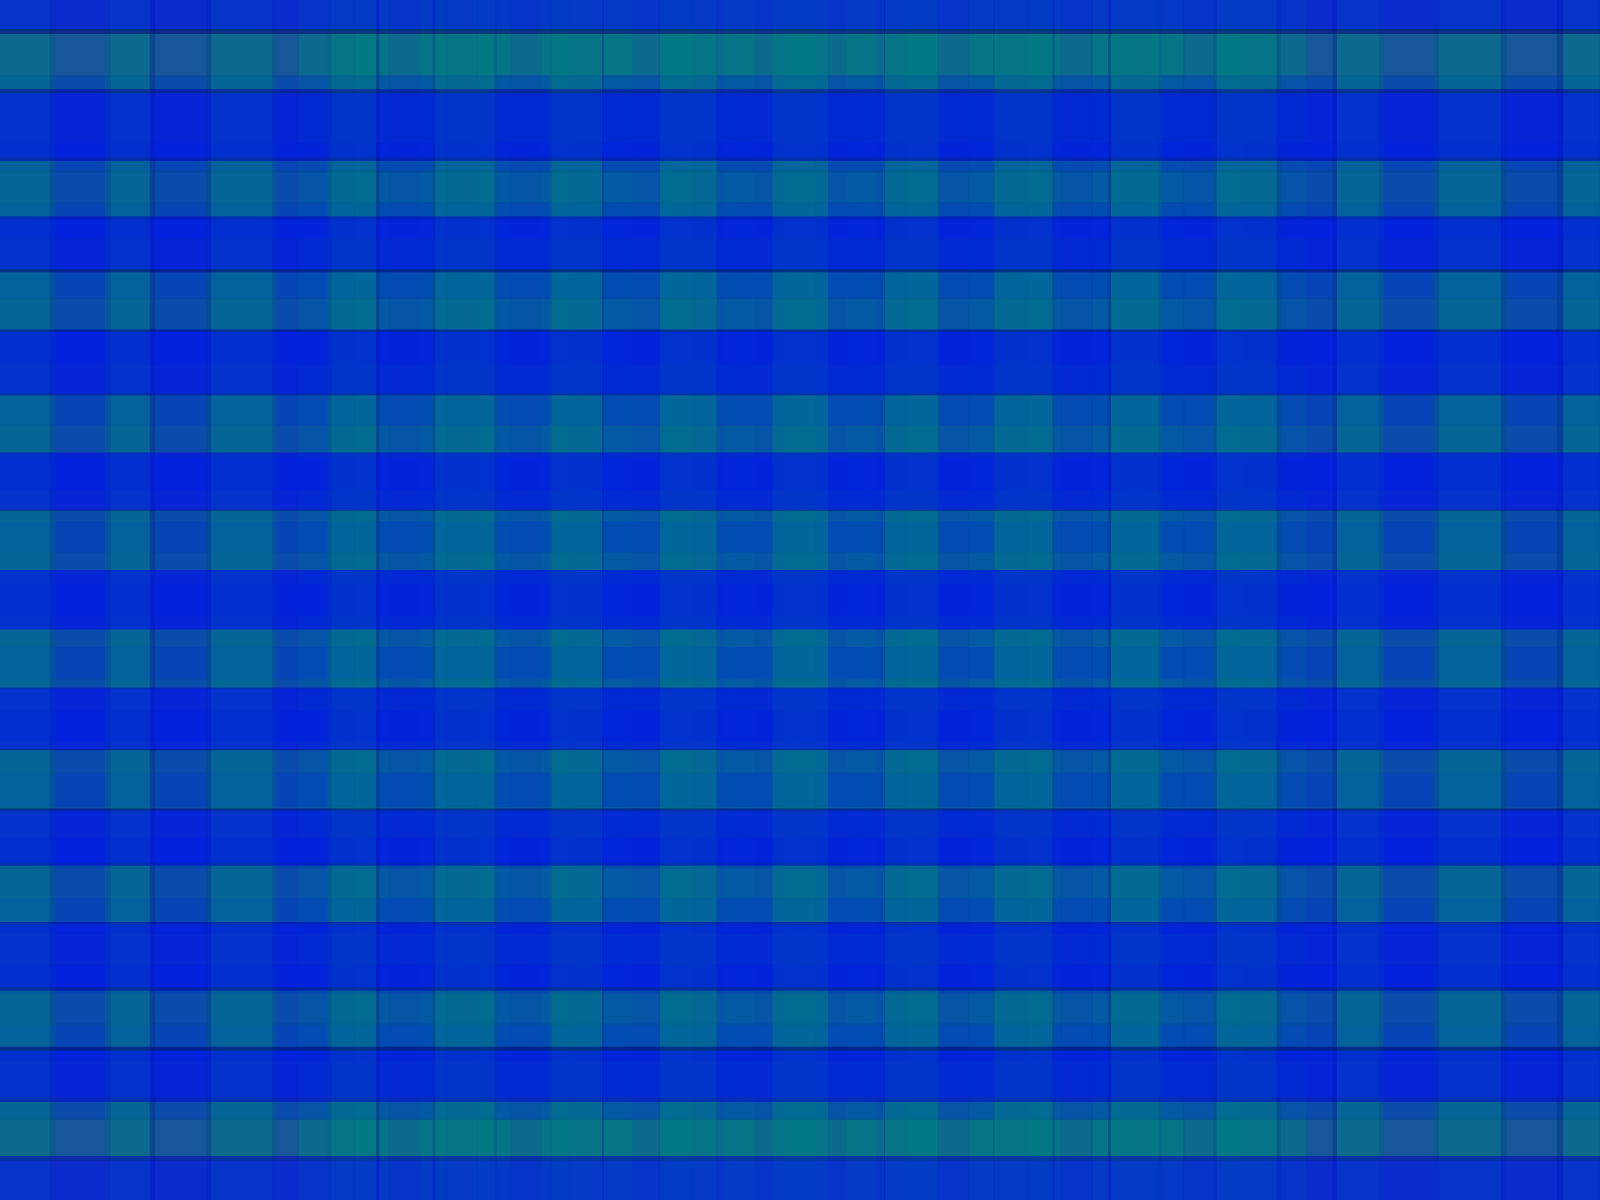
\includegraphics[height=0.78\textheight]{figures/meiga_geometry_view.png}

  \vspace{0.4em}
  \small Vista renderizada automáticamente desde el WRL exportado por Meiga/Geant4.
\end{frame}
}{
% No se encontró figures/meiga_geometry_view.png.
% La escena WRL queda disponible en figures/meiga_geometry_raw/g4_00.wrl.
% Puede renderizarse manualmente y guardarse como figures/meiga_geometry_view.png.
}

\IfFileExists{figures/meiga_trajectories_view.png}{
\begin{frame}{Trayectorias simuladas}
  \centering
  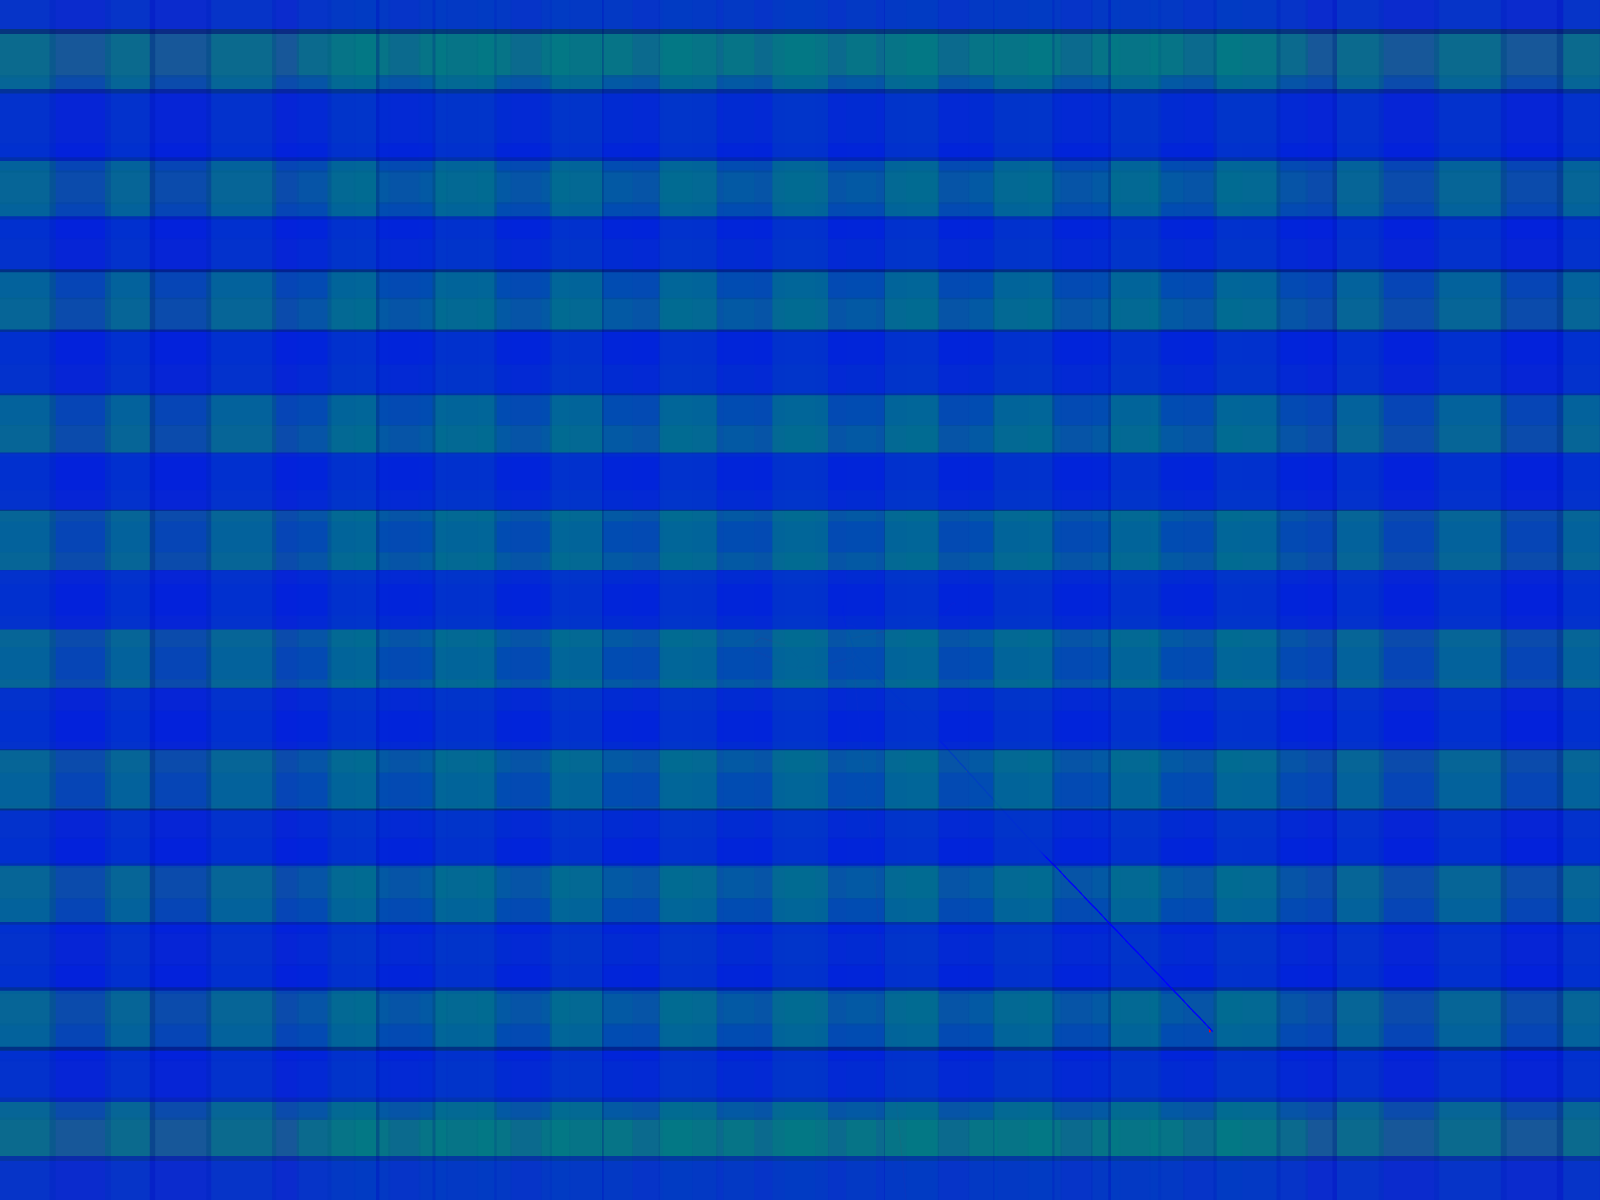
\includegraphics[height=0.78\textheight]{figures/meiga_trajectories_view.png}

  \vspace{0.4em}
  \small Vista renderizada desde \code{g4\_trajectories.wrl}, si está disponible.
\end{frame}
}{
% No se encontró figures/meiga_trajectories_view.png.
% Si existe g4_trajectories.wrl, render_meiga_geometry.sh intentará generar esta imagen.
}

\begin{frame}{Interpretación}
  \begin{itemize}
    \item La geometría implementada reproduce la segmentación esperada: dos módulos, 64 barras activas y 256 píxeles por módulo.
    \item Las coincidencias completas aparecen en una fracción significativa de eventos: 567 de 1000.
    \item La multiplicidad 2 es consistente con zonas de overlap y subplanos desplazados.
    \item La salida ya permite construir píxeles discretos y avanzar hacia reconstrucción angular.
  \end{itemize}
\end{frame}

\begin{frame}{Limitaciones actuales}
  \begin{itemize}
    \item Modo de material muerto: \code{active\_only}.
    \item Reflectores tratados como metadatos; material pasivo simplificado pendiente.
    \item Sin generación ni transporte completo de fotones ópticos.
    \item Sin respuesta realista de SiPM.
    \item Sin pulsos electrónicos, jitter ni electrónica CAEN.
    \item Sin matriz \(F\) final ni reconstrucción tomográfica completa.
  \end{itemize}
\end{frame}

\begin{frame}{Próximos pasos}
  \begin{enumerate}
    \item Iteración 2: material muerto simplificado.
    \item Iteración 3: respuesta óptica parametrizada.
    \item Iteración 4: SiPM, pulsos y electrónica.
    \item Iteración 5: reconstrucción angular y matriz \(F\).
  \end{enumerate}

  \vspace{1em}
  \begin{block}{Estado actual}
    La base activa está validada: geometría, scoring por barra, píxeles discretos
    y coincidencias LOWER-UPPER.
  \end{block}
\end{frame}

\end{document}
